\documentclass[english, aspectratio=169]{beamer}
% english is for the language used in standard texts (figures, tables etc)
% aspectratio of 16:9 or set it for more old school to 4:3 (without the ':')

% ---------------------------------------------------------------------------- %
% Load base preamble
% ---------------------------------------------------------------------------- %
\usepackage{import}
\subimport{./preamble/}{beamer.tex}

% ---------------------------------------------------------------------------- %
% Local settings
% ---------------------------------------------------------------------------- %
\usepackage{ulem}

% ------------------------------------------------------------------------------
% TITLEPAGE
% ------------------------------------------------------------------------------
\title{Efficient Dependency Resolution\\in IFC-aware Decentralized Programming}

\author{\textbf{Steffan Christ S\o lvsten} and Aslan Askarov}

\institute{
\includegraphics[width=0.2\linewidth]{external/aulogo_uk_var2_black.eps}}

\date{PRiSC 2026}

\begin{document}

\titleframe

% ------------------------------------------------------------------------------
% Goal: Resource Reuse
% - Fig 1: The goal, Demo
% - Fig 2 (confidentiality): Demo
% - Fig 3 (integrity): Demo
% - Fig 4 (availability): Demo

\begin{frame}
  \frametitle{\quad}%{Resource Reuse}

  \begin{figure}
    \centering\huge

    \begin{tikzpicture}[scale=2]
      \node[shape=rectangle, draw=black] at (0, 0)
      (A) {\texttt{A}};

      \node[shape=rectangle, draw=black] at (4, 0)
      (B) {\texttt{B}};

      \onslide<2-> {
        \draw[->] (A) edge node[above] {$f_M$} (B);
      }
      \onslide<3-> {
        \draw[->] (A) edge[bend right=30] node[below] {$g_M$} (B);
      }
    \end{tikzpicture}

    % \caption{Figure 1: Resource Reuse\footnotemark.}
  \end{figure}

  \footnotetext[1]{Using hashes to uniquely identify an object/class is called a
    ``\textit{fingerprint}'' in\\O. Arden et al. \textit{Sharing Mobile Code
      Securely with Information Flow Control} (2012).}

  \setcounter{footnote}{1}
\end{frame}

\begin{frame}
  \frametitle{Leaky Cache\footnotemark\ (Confidentiality)}

  \begin{figure}
    \centering\huge

    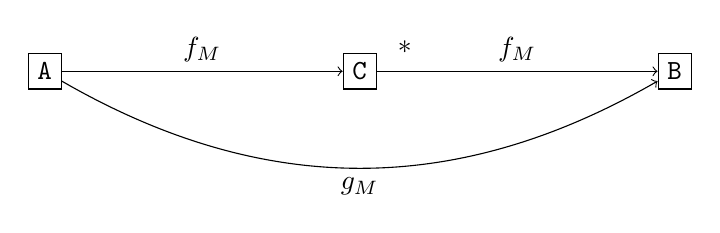
\begin{tikzpicture}[scale=2]
      \node[shape=rectangle, draw=black] at (0, 0)
      (A) {\texttt{A}};

      \node[shape=rectangle, draw=black] at (2, 0)
      (C) {\texttt{C}};

      \node[shape=rectangle, draw=black] at (4, 0)
      (B) {\texttt{B}};

      \onslide<2-> {
        \draw[->] (A) edge node[above] {$f_M$} (C);
      }
      \onslide<3-> {
        \draw[->] (C) edge node[above, pos=.1] {*} node[above] {$f_M$} (B);
      }
      \onslide<4-> {
        \draw[->] (A) edge[bend right=30] node[below] {$g_M$} (B);
      }
    \end{tikzpicture}

    % \caption{Figure 2: Leaky Cache.}
  \end{figure}

  \footnotetext[2]{This behaviour is a remanifestation of a ``\textit{read
      channel}'' in\\O. Arden et al. \textit{Sharing Mobile Code Securely with
      Information Flow Control} (2012).}
\end{frame}

\begin{frame}
  \frametitle{Replay Dependency\footnotemark\ (Integrity)}

  \begin{figure}
    \centering\huge

    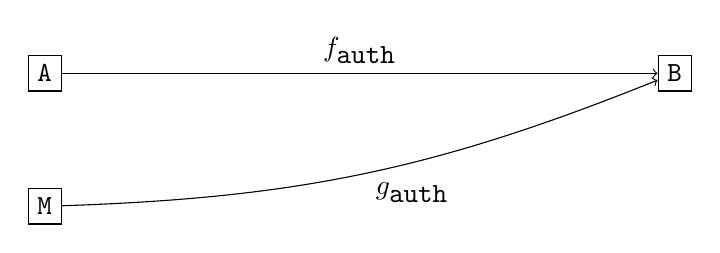
\begin{tikzpicture}
      \node[shape=rectangle, draw=black] at (0, 0)
      (A) {\texttt{A}};

      \node[shape=rectangle, draw=black] at (8, 0)
      (B) {\texttt{B}};

      \draw[->]
        % A -> B
        (A) edge node[above] {$f_{\texttt{auth}}$} (B)
      ;

      \onslide<2-> {
        \node[shape=rectangle, draw=black] at (0,-1.69)
        (M) {\texttt{M}};

        \draw[->]
          % C -> B
          (M) edge[bend right=10] node[below right] {$g_{\texttt{auth}}$} (B)
        ;
      }
    \end{tikzpicture}

    %\caption{Figure 3: Replay Dependency.}
  \end{figure}

  \footnotetext[3]{This behavior is a remanifestation of the
    ``\textit{provider-bounded authority}'' requirement in\\O. Arden et al.
    \textit{Sharing Mobile Code Securely with Information Flow Control} (2012).}
\end{frame}

\begin{frame}
  \frametitle{Chain of Death\footnotemark\ (Availability)}

  \begin{figure}
    \centering\huge

    \begin{tikzpicture}[scale=2]
      % A -> B
      \node[shape=rectangle, draw=black] at (0, 0)
      (A) {\texttt{A}};

      \onslide<2-> {
        \node[shape=rectangle, draw=black] at (1, 0)
        (B) {\texttt{B}};

        \draw[->] (A) edge[bend left] node[above] {$f_M$} (B);
      }
      \onslide<3-> {
        \node at (0, -1) (Ad) {$\dagger$};
        \draw[->] (A) edge[dashed] (Ad);
      }

      % B -> C
      \onslide<4-> {
        \node[shape=rectangle, draw=black] at (2, 0)
        (C) {\texttt{C}};

        \draw[->] (B) edge[bend left] node[above] {$f_M$} (C);
      }
      \onslide<5-> {
        \node at (1, -1) (Bd) {$\dagger$};
        \draw[->] (B) edge[dashed] (Bd);
      }

      % C -> ...
      \onslide<6-> {
        \node at (3, 0)   (D) {\quad};
        \node at (3.5, 0) (dots) {\dots};

        \draw[->] (C) edge[bend left] node[above] {$f_M$} (D);
      }
      \onslide<7-> {
        \node at (2, -1) (Cd) {$\dagger$};
        \draw[->] (C) edge[dashed] (Cd);
      }

      % ... -> Z
      \onslide<8-> {
        \node at (4, 0)   (Y) {\quad};
        \node[shape=rectangle, draw=black] at (5, 0)
        (Z) {\texttt{Z}};

        \draw[->] (Y) edge[bend left] node[above] {$f_M$} (Z);
      }
      \onslide<9-> {
        \node at (5, -1) (Zf) {$f_M()$};
        \draw[->] (Z) edge[dashed] (Zf);
      }
    \end{tikzpicture}

    %\caption{Figure 4: Chain of Death.}
  \end{figure}

  \footnotetext[4]{This is related to the notion of ``\textit{mobile code}''. But,
    code should outlive its origin, i.e.\ be \textit{nomadic}.\\O. Arden et
    al. \textit{Sharing Mobile Code Securely with Information Flow Control}
    (2012)}
\end{frame}

\begin{frame}[plain,noframenumbering]
  \begin{center}
    \onslide<1->{
      \LARGE\bf

      How can one add IFC-aware caching?
    }

    \onslide<2->{
      \large\bf

      (with the minimal extension to the TCB\dots)
    }
  \end{center}
\end{frame}

% ------------------------------------------------------------------------------
% Troupe Programming Language
% - Decentralized Programming
% - Information Flow Control
% - Dynamically Typed

\begin{frame}[fragile]
  \frametitle{Troupe Programming Language}

  \begin{columns}
    \begin{column}{0.45\linewidth}
      {\color{gray} \texttt{(* Alice.trp *)}}
      \begin{lstlisting}[language=troupe]
let val msg = "Hello, Bob!"
    fun f () = print msg
in send (@bob, f)
end
      \end{lstlisting}

      {\color{gray} \texttt{(* Bob.trp *)}}
      \begin{lstlisting}[language=troupe, firstnumber=last]
let fun loop () =
    receive [hn f => spawn f];
    loop ()
in loop ()
end
      \end{lstlisting}
    \end{column}
    \begin{column}{0.55\linewidth}
      \begin{itemize}
      \item \textbf{Decentralized Programming}

        For creation of open self-organizing distributed systems.

      \item \textbf{Information Flow Control}

        Ensures secret information is not by accident shared with nor affected
        by unwanted parties.

      \item \textbf{Dynamically Typed}

        Permits the dynamic behaviour needed by a truly open and updateable
        system.

      \end{itemize}
    \end{column}
  \end{columns}
\end{frame}

% ------------------------------------------------------------------------------
% Requirements on the HashMap
% - Implemented in Troupe itself (to not increase the TCB)
% => Expand Figure 1
% - Mitigate timing attacks
% => Use Troupe's sandboxing feature
% - Resources should be (carefully) reused across levels
% => secret key-value pairs should not taint public ones
% => level-based view of history

\begin{frame}[plain,noframenumbering]
  \begin{center}
    {
      \LARGE\bf\only<2->{\color{lightgray}}

      How can one add IFC-aware caching?
    }

    {
      \large\bf

      (with the minimal extension to the TCB\dots)
    }
  \end{center}
\end{frame}

\begin{frame}
  \begin{figure}
    \centering

    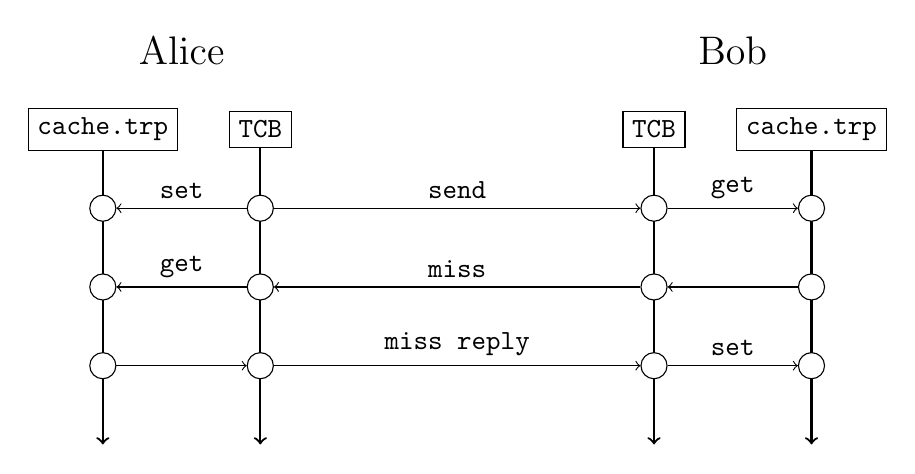
\begin{tikzpicture}
      \node at (1,1) {\Large Alice};
      \node[draw=black] at (0,0) (A-cache) {\texttt{cache.trp}};
      \node[draw=black] at (2,0) (A-p2p) {\texttt{TCB}};

      \node at (8,1) {\Large Bob};
      \node[draw=black] at (7,0) (B-p2p) {\texttt{TCB}};
      \node[draw=black] at (9,0) (B-cache) {\texttt{cache.trp}};

      \draw[->, thick]
        (A-cache) edge ++(0,-4)
        (A-p2p)   edge ++(0,-4)
        (B-p2p)   edge ++(0,-4)
        (B-cache) edge ++(0,-4)
      ;

      \onslide<2-> {
        \node[shape=circle, draw=black, fill=white] (AP-1) at (2,-1) {};
        \node[shape=circle, draw=black, fill=white] (AC-1) at (0,-1) {};
        \node[shape=circle, draw=black, fill=white] (BP-1) at (7,-1) {};

        \draw[->] (AP-1) edge node[above] {\texttt{set}} (AC-1);
        \draw[->] (AP-1) edge node[above] {\texttt{send}} (BP-1);
      }
      \onslide<3-> {
        \node[shape=circle, draw=black, fill=white] (BC-1) at (9,-1) {};
        \draw[->] (BP-1) edge node[above] {\texttt{get}} (BC-1);
      }
      \onslide<4-> {
        \node[shape=circle, draw=black, fill=white] (BC-2) at (9,-2) {};
        \node[shape=circle, draw=black, fill=white] (BP-2) at (7,-2) {};

        \draw[->] (BC-2) edge (BP-2);
      }
      \onslide<5-> {
        \node[shape=circle, draw=black, fill=white] (AP-2) at (2,-2) {};

        \draw[->] (BP-2) edge node[above] {\texttt{miss}} (AP-2);
      }
      \onslide<6-> {
        \node[shape=circle, draw=black, fill=white] (AC-2) at (0,-2) {};
        \node[shape=circle, draw=black, fill=white] (AC-3) at (0,-3) {};
        \node[shape=circle, draw=black, fill=white] (AP-3) at (2,-3) {};
        \node[shape=circle, draw=black, fill=white] (BP-3) at (7,-3) {};

        \draw[->] (AP-2) edge node[above] {\texttt{get}} (AC-2);
        \draw[->] (AC-3) edge (AP-3);
        \draw[->] (AP-3) edge node[above] {\texttt{miss reply}} (BP-3);
      }
      \onslide<7-> {
        \node[shape=circle, draw=black, fill=white] (BC-3) at (9,-3) {};
        \draw[->] (BP-3) edge node[above] {\texttt{set}} (BC-3);
      }
    \end{tikzpicture}

    % \caption{Figure 1*: Resource Reuse}
  \end{figure}
\end{frame}

\begin{frame}
  \frametitle{Changes to Runtime (TCB)}
  \begin{itemize}
  \item {\bf Peer-to-peer layer:}

    Extend with \texttt{miss} and \texttt{miss reply} messages. Unlike
    \texttt{send}, these should always be sent by value.

  \item {\bf Serialization:}

    Dependency resolution requires introspection of function closures.
    \begin{itemize}
    \item During \texttt{serialize}, identify (sub)values to be referenced by hash.

    \item To \texttt{deserialize}, (1) extract references (2) deserialize given
      (all resolved) dependencies.
    \end{itemize}

  \item {\bf Hash:}

    Hashing Troupe values requires introspection of function closures and definition.

  \item {\bf Scheduler:}

    Extend to run Troupe code from the peer-to-peer layer.
  \end{itemize}
\end{frame}

\begin{frame}[t]
  \frametitle{Additions in Troupe: IFC-aware \texttt{Map} / \texttt{HashMap}}

  \vspace{-20pt}
  \begin{align*}
      A &\xrightarrow{m@\{A\}} B \implies \text{miss}
    & C &\xrightarrow{m@\{\}}  B \implies \text{miss}
    & D &\xrightarrow{m@\{D\}} B \onslide<2->{\implies \text{hit}}
  \end{align*}

  \onslide<3->{
    \textbf{``Specification'':}

    \vspace{-6pt} An IFC-aware \texttt{HashMap} is a single data structure with
    public and secret key-value pairs which provides a IFC-aware projections of
    its \texttt{insert} and \texttt{remove}\footnotemark\ history:

    \vspace{-20pt}
    \begin{center}
      \begin{tabular}{cccccc}
        \texttt{i($x \mapsto 1$)@\{\}}, &
        \only<4,6>{\color{lightgray}}\texttt{i($x \mapsto 2$)@\{A\}}, &
        \only<4-5>{\color{lightgray}}\texttt{i($y \mapsto 3$)@\{B\}}, &
        \only<4-5>{\color{lightgray}}\texttt{r($x$)@\{B\}}, &
        \texttt{i($y \mapsto 4$)@\{\}}, &
        $\dots$
      \end{tabular}

      \vspace{-5pt}
      \onslide<4->{
        $\shortparallel$\,\,\\
        {\large
          \only<1-4>{\texttt{@\{\}}\\}%
          \only<5>{\texttt{@\{A\}}\\}%
          \only<6>{\texttt{@\{B\}}\\}
        }
        $\Downarrow$
      }

      \vspace{-5pt}
      \onslide<4->{ \large
        \only<1-4>{\texttt{[$x \mapsto 1$@\{\}, $y \mapsto 4$@\{\}] @\{\}}}%
        \only<5>{\texttt{[$x \mapsto 2$@\{A\}, $y \mapsto 4$@\{\}] @\{A\}}}%
        \only<6>{\texttt{[$y \mapsto 4$@\{\}] @\{B\}}}%
      }
    \end{center}
  }

  \footnotetext[\number\value{footnote}]<3->{For this particular use case, we
    actually only need public ( \texttt{@\{\}} ) \texttt{remove} operations.}
\end{frame}


\begin{frame}
  \frametitle{Additions in Troupe: caching layer}

  55~LOC to orchestrate a \texttt{HashMap} instance:
  \begin{itemize}
  \item Hash function for \texttt{HashMap}: SHA256 \texttt{string}
    $\rightarrow$ 32-bit \texttt{int}. (4~LOC)

  \item Define and spawn a local Troupe thread to manage the \texttt{HashMap}
    instance. (26~LOC)

  \item Define and export \texttt{set} and \texttt{get} functions callable
    from the TCB. (8~LOC)

  \item Wrapper on \texttt{sandbox} builtin. (14~LOC)
  \end{itemize}

  Initialize twice in the TCB for the sender and receiver caches.
\end{frame}

\begin{frame}[fragile]
  \frametitle{Additions in Troupe: caching layer (timing-attack mitigation)}

  Troupe provides the \texttt{{\color{blue} sandbox}($f$, $t$)} operation to run
  $f$ for $t$~ms and either return the result, an error, or a continuation. In
  practice, $t = 1$~ms seems to suffice.

  \begin{lstlisting}[language=troupe, numbers=none]
(* cache.trp : line 48 *)
val (m, t') =
    *@sandbox'@* (fn () => HashMap.insert  m auth k v) t m
  \end{lstlisting}
  \begin{lstlisting}[language=troupe, numbers=none]
(* cache.trp : line 57 *)
val (v, t') =
    *@sandbox'@* (fn () => HashMap.findAll m auth k)   t []
  \end{lstlisting}
\end{frame}

% ------------------------------------------------------------------------------

\begin{frame}[plain,noframenumbering]
  \begin{center}
    {
      \LARGE\bf

      How can one add IFC-aware caching?
    }

    \onslide<2->{
      \large\bf

      By bootstrapping the IFC-aware runtime!
    }
  \end{center}
\end{frame}

\begin{frame}[plain,noframenumbering]
  % custom copy of fram/endslate.tex
  \begin{columns}
    \begin{column}{0.43\linewidth}
      {\Large \textbf{Steffan Christ S{\o}lvsten}}
      \vspace{1pt} {\hrule width\linewidth}

      \vspace{5pt}

      \begin{itemize}
      \item[\faIcon{envelope}] \mailto{soelvsten@cs.au.dk}
      \item[\faIcon{globe}] \href{https://ssoelvsten.github.io}{ssoelvsten.github.io}
      \end{itemize}

      \vspace{10pt}

      {\Large \textbf{Troupe}}
      \vspace{1pt} {\hrule width\linewidth}

      \vspace{5pt}

      \begin{itemize}
      \item[\faIcon{code}]
        \href{http://github.com/TroupeLang/troupe}{github.com/TroupeLang/troupe}
      \end{itemize}

      \vspace{10pt}

      
\includegraphics[width=0.5\linewidth]{external/aulogo_uk_var2_black.eps}
    \end{column}
    \begin{column}{0.56\linewidth}
    \end{column}
  \end{columns}
\end{frame}

% ------------------------------------------------------------------------------
\blankframe

\begin{frame}
  \frametitle{Troupe's Threat Model}

  Uses several security mechanisms, inspired by Jif, Fabric, and FLAM.
  \begin{itemize}
  \item Progress-sensitive Dynamic Information-flow Control
  \item Sandboxing
  \item Capabilities
  \end{itemize}

  Few assumptions on adversaries! But, we do ignore:
  \begin{itemize}
  \item Network Traffic Analysis. Can be avoided with via recent methods.\\
    {\footnotesize (Blaabjerg and Askarov '21 \& '23, Nelson, Pagnin, and Askarov '24)}
  \item Timing-channels. Can be avoided via \texttt{sandbox}ing and predictive
    mitigation.
    {\footnotesize (Zhang, Askarov, Myers '10 \& '12)}
  \end{itemize}
\end{frame}

% ------------------------------------------------------------------------------
\blankframe

\begin{frame}
  \frametitle{Design of the \texttt{HashMap}}

  \begin{columns}
    \begin{column}{0.5\linewidth}
      Current prototype uses a Hash Array Mapped Trie (HAMT) with 200~LOC.

      \bigskip

      Only 3 declassifications per \texttt{insert}, \texttt{remove},
      \texttt{find} (--24/+55~LOC):
      \begin{itemize}
      \item \texttt{hash key} and \texttt{hash bucket} to not raise \texttt{pc}
        and taint the entire trie.
      \item The \texttt{bucket} list (but not its content).
      \end{itemize}

      But, this fully declassifies its \texttt{size}!
    \end{column}
    \begin{column}{0.49\linewidth}
      \centering

      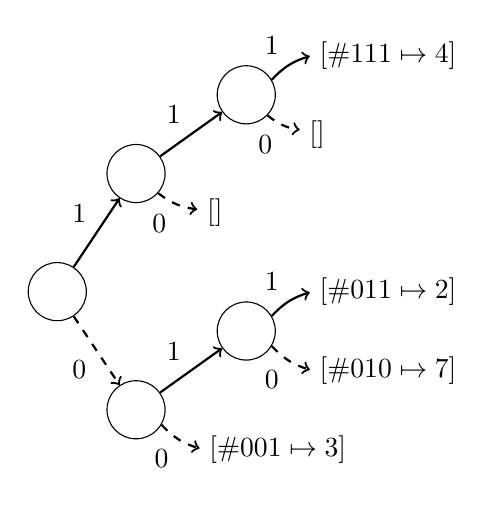
\begin{tikzpicture}
        \tikzstyle{trie_node} = [shape = circle,    draw = black, minimum size=21pt]
        \tikzstyle{trie_leaf} = []

        \node[trie_node] at (0.0,  0.0) (n1) {};

        \node[trie_node] at (1,  1.5) (n2) {};

        \node[trie_leaf] at (2,  1.0) (n2_l1) {$[]$};

        \node[trie_node] at (2.4,  2.5) (n3) {};

        \node[trie_leaf] at (4.2,  3.0) (n3_l1) {$[ \#111 \mapsto 4 ]$};

        \node[trie_leaf] at (3.3,  2.0) (n3_l2) {$[]$};

        \node[trie_node] at (1, -1.5) (n4) {};

        \node[trie_leaf] at (2.8, -2.0) (n4_l1) {$[ \#001 \mapsto 3 ]$};

        \node[trie_node] at (2.4, -0.5) (n5) {};

        \node[trie_leaf] at (4.2,  0.0) (n5_l1) {$[ \#011 \mapsto 2 ]$};

        \node[trie_leaf] at (4.2, -1.0) (n5_l2) {$[ \#010 \mapsto 7 ]$};

        \draw[->, dashed, thick]
          (n1) edge node[below left] {0} (n4)
          (n2) edge[bend right=15] node[below left] {0} (n2_l1)
          (n3) edge[bend right=15] node[below left] {0} (n3_l2)
          (n4) edge[bend right=15] node[below left] {0} (n4_l1)
          (n5) edge[bend right=15] node[below left] {0} (n5_l2)
        ;

        \draw[->, thick]
          (n1) edge node[above left] {1} (n2)
          (n2) edge node[above left] {1} (n3)
          (n3) edge[bend left=15] node[above left] {1} (n3_l1)
          (n4) edge node[above left] {1} (n5)
          (n5) edge[bend left=15] node[above left] {1} (n5_l1)
        ;
      \end{tikzpicture}
    \end{column}
  \end{columns}
\end{frame}

\begin{frame}
  \frametitle{Design of the \texttt{HashMap}}

    \begin{columns}
    \begin{column}{0.5\linewidth}
      Can we design a meta data structure for \texttt{HashMap} and \texttt{Map}?

      \begin{itemize}
      \item<2-> Guard taint of secret sub structures with (first-class) IFC labels.
      \item<3-> Use the partial ordering on information flow ($\sqsubseteq$) to
        compare levels.
      \item<4-> Use buffers to accumulate operations for ``inaccessible'' sub
        structures. This keeps \texttt{insert} and \texttt{remove} efficient.
      \item<5-> Use time-stamps to identify latest key-value from sub structures.
      \end{itemize}

      \onslide<5->{But, does this make \texttt{find} too slow?}
    \end{column}
    \begin{column}{0.49\linewidth}
      \centering

      \begin{tikzpicture}
        \tikzstyle{tree_node} = [shape = circle, draw = black, minimum size=21pt]
        \tikzstyle{buffer} = []

        \node at (0, 2) (p) {};
        \node[tree_node] at (0,   0) (n) {$@\{\dots\}$};

        \draw[->, thick] (p) edge (n);

        \onslide<2-> {
          \node at (3, 0) (ds) {$\dots$};
          \draw[->, dashed, thick]
            (n) edge node[above] {$=$} (ds)
          ;
        }
        \onslide<3-> {
          \node[tree_node] at (-2, -3) (nLt) {};
          \node[tree_node] at ( 0, -3) (nNc) {};
          \node[tree_node] at ( 2, -3) (nGt) {};

          \draw[->, thick]
            (n) edge node[above left]  {$\sqsubset$} (nLt)
            (n) edge node[above right] {$\sqsupset$} (nGt)
            (n) edge node[above left] {$?$} (nNc)
          ;
        }
        \onslide<4-> {
          \node[buffer] at (1.7,1) {\small $[i(k,v), r(k), \dots]$};
        }
      \end{tikzpicture}
    \end{column}
  \end{columns}
\end{frame}

\end{document}